\newpage
%%%%%%%%%%%%%%
\section{Evaluaci\' on}
%%%%%%%%%%%%%%

\par Para evaluar las pruebas planteadas en el apartado anterior, se ejecutaron los bancos de pruebas y se graficaron las se\~ nales resultantes (archivo signals.vcd), para analizar los resultados obtenidos.
\\
\par En los siguientes apartados se muestran los resultados obtenidos para cada uno de los multiplicadores.

\subsection{Banco de pruebas del decodificador de instrucciones}
El decodificador de instrucciones es el m\' odulo que se encarga de ajustar todas las se\~ nales de control del procesador de acuerdo a la instrucci\' on que se est\' a procesando en cada ciclo de reloj, de manera tal que debe ser capaz de obtener la decodificaci\' on de la instrucci\' on, las se\~ nales de control: \textit{write to a, write to b, mux pre alu a, mux pre alu b, read write, write back mux, jump, write mux y branch taken} de acuerdo al avance del contador de programa \textit{pc}.

Es de esta manera como se realiz\' o la simulaci\' on de las instrucciones que modifican las se\~ nales de control y se puede observar en la Figura \ref{fig:decoder} como efectivamente se tienen los resultados esperados de acuerdo con el dise\~ no del procesador.

\begin{figure}[hbtp]
\caption{Simulaci\' on del decodificador de instrucciones}
\centering
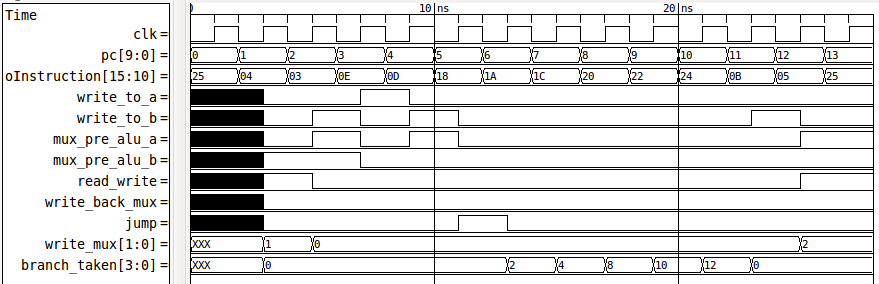
\includegraphics[scale=0.6]{../Codes/Verilog_Testbenches/scopes/Decoder_scope.png}
\label{fig:decoder}
\end{figure}


\subsection{Banco de pruebas de la ALU}
El m\' odulo ALU es el que se encarga de realizar el c\' alculo aritm\' etico de ciertas instrucciones que lo requieren y adem\' as obtener el valor de la se\~ nal de carry y la se\~ nal de cero. Tambien se encarga de realizar el c\' alculo de las direcciones de memoria para instrucciones que tienen que ver con el acceso o ingreso a la memoria principal.

De acuerdo con lo anterior y con la descripci\' on proporcionada en la secci\' on de dise\~ no se puede observar los resultados de la simulaci\' on efectuada en la Figura \ref{fig:alu} donde cabe destacar que el valor de los operandos \textit{in1, in2} y el resultado final \textit{out} se observa en formato decimal, mientras que las se\~ nales de \textit{carry} y \textit{zero} son bits.


\begin{figure}[hbtp]
\caption{Simulaci\' on de m\' odulo alu}
\centering
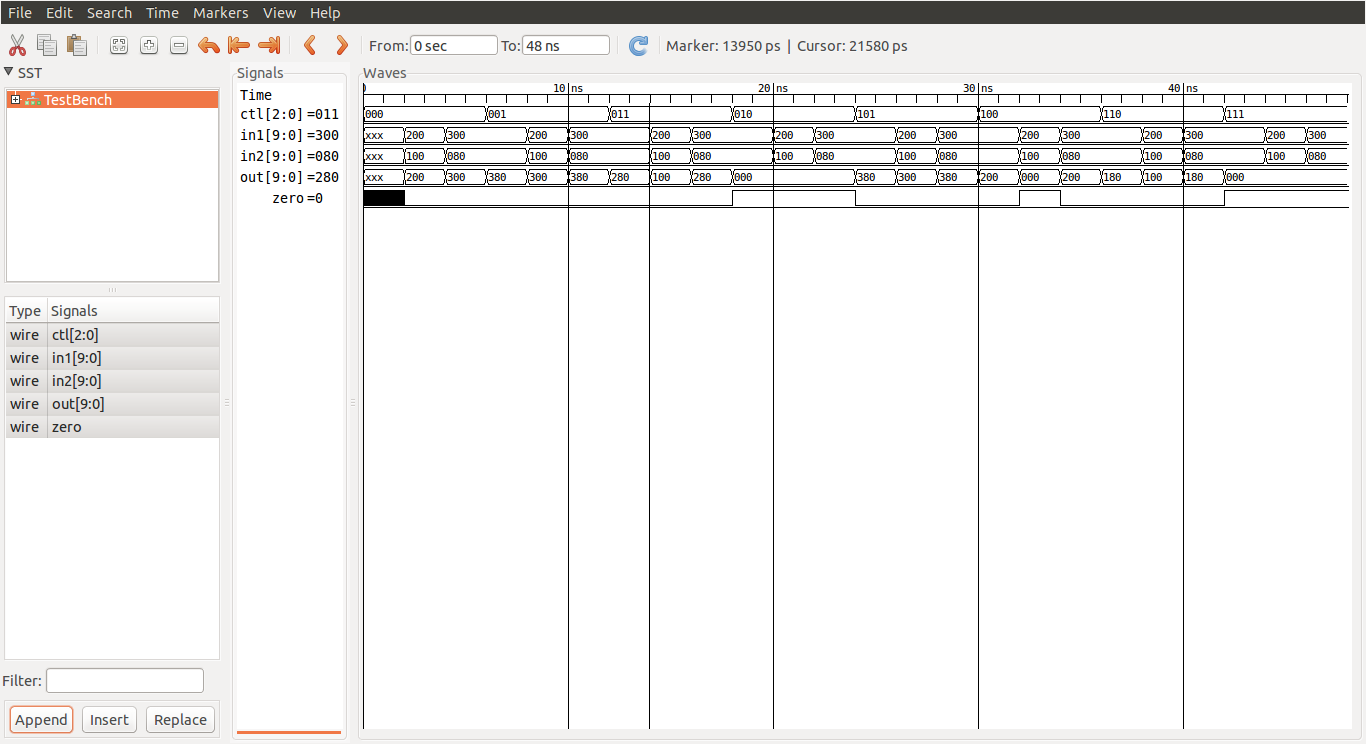
\includegraphics[scale=0.48]{../Codes/Verilog_Testbenches/scopes/ALU.png}
\label{fig:alu}
\end{figure}

\subsection{Banco de pruebas del controlador de ALU}
El m\' odulo controlador de la ALU es bastante importante en tanto que se encarga de obtener los bits de control que se encargan de decirle al m\' odulo ALU la tarea que debe desarrollar, por lo que en la evaluaci\' on de este m\' odulo se debe de tener como entrada todas las posibles instrucciones que se pueden ejecutar en el procesador y obtener a partir del c\' odigo de instrucci\' on, el c\' odigo de operando que debe implementar la ALU.

El resultado de la simulaci\' on se puede observar en la Figura \ref{fig:aluControl} donde se puede destacar que los c\' odigos de presentan en formato octal y adem\' as en orden de acuerdo con la descripci\' on presentada en la secci\' on de dise\~ no.

\begin{figure}[hbtp]
\caption{Simulaci\' on de m\' odulo controlador de alu}
\centering
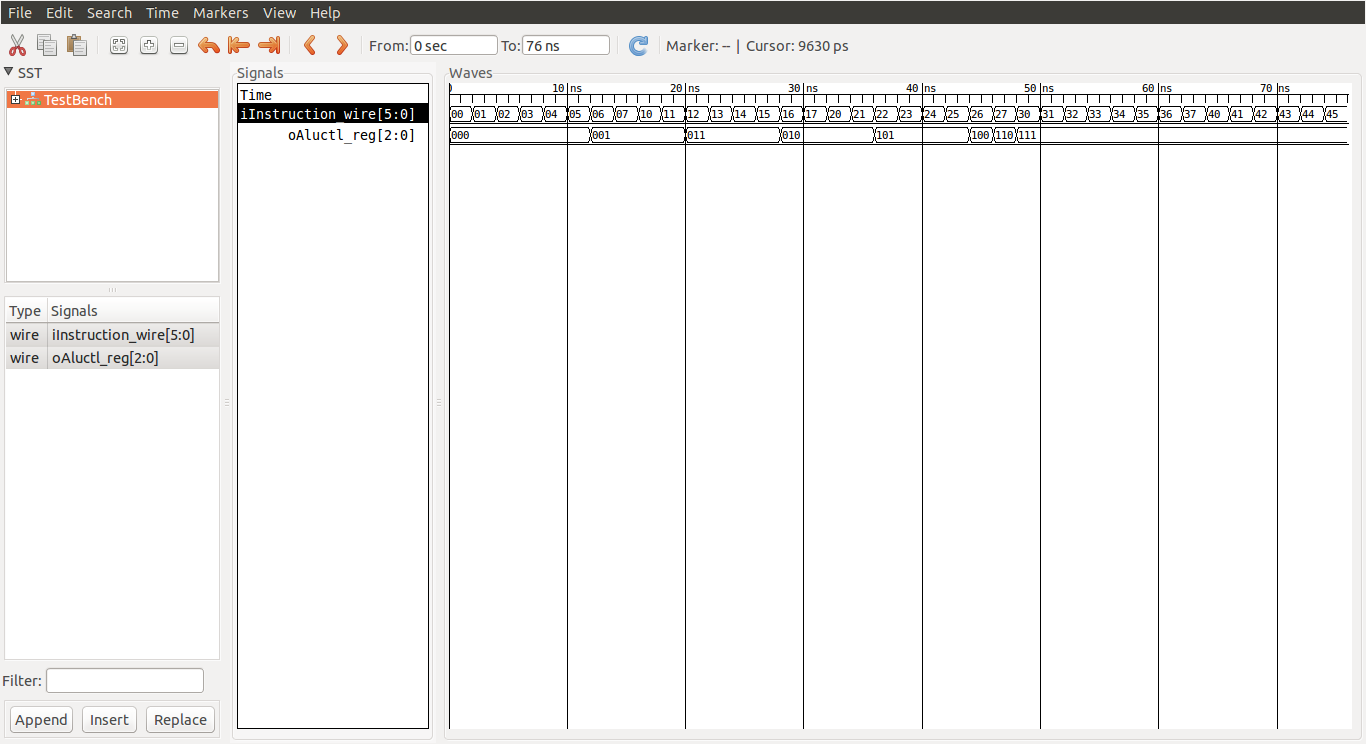
\includegraphics[scale=0.48]{../Codes/Verilog_Testbenches/scopes/ALU_Controller_scope.png}
\label{fig:aluControl}
\end{figure}


\subsection{Banco de pruebas del m\' odulo \textit{branch taken}}

\subsection{Banco de pruebas de las memorias}




